\documentclass[./../Technology Baseline.tex]{subfiles}

\begin{document}
	
\chapter{Tecnologie selezionate}
	
\section{Introduzione}
In questo capitolo vengono esposte e motivate le principali tecnologie, framework e librerie selezionati per lo sviluppo \textit{DeSpeect}.

\section{Classificazione delle tecnologie}

A fini di tracciabilità, le tecnologie di seguito esposte vengono catalogate secondo il seguente codice:

\begin{center}
	T[Categoria][ID]
\end{center}

Dove:

\begin{itemize}
	\item \textbf{T}: indica che si tratta di una tecnologia;
	\item \textbf{Categoria}: indica la categoria a cui appartiene la tecnologia in esame. Può assumere i seguenti valori:
		\begin{itemize}
			\item \textbf{S}: indica che la tecnologia è inerente lo \textit{sviluppo} del prodotto;
			\item \textbf{O}: indica che la tecnologia è inerente l'\textit{organizzazione} del gruppo.
		\end{itemize}
	\item \textbf{ID}: rappresenta un codice numerico incrementale atto all'identificazione univoca della tecnologia.
\end{itemize}

\noindent Le tecnologie sono presentate secondo il seguente schema: 

\begin{itemize}
	\item Codice - Nome e versione (ove possibile);
	\item Descrizione e contesto di utilizzo;
	\item Motivazioni generali della scelta e tecnologie concorrenziali;
	\item Dimostrazione di adeguatezza rispetto agli obiettivi di prodotto:
	\begin{itemize}
		\item Considerazioni generali;
		\item Competenza del gruppo;
		\item Usabilità;
		\item Costo economico;
		\item Consumo di risorse;
		\item Sviluppi possibili della tecnologia.
	\end{itemize}
	\item \textit{Proof of Concept} (laddove lo si ritenga necessario);
	\item Aspetti negativi.
\end{itemize}

\section{Tecnologie inerenti lo sviluppo del prodotto}

\subsection{TS01 - Speect v1.1.0-69-g65f4}

\subsubsection{Descrizione e contesto di utilizzo}

Speect è un sistema di \textit{Text To Speech} (TTS) multilingua. Esso offre un sistema TTS completo (analisi e decodifica del testo e sintesi vocale) con annesse varie API, nonché un ambiente per la ricerca e lo sviluppo di sistemi e voci TTS. Speect è scritto in linguaggio C, con una stretta conformità allo standard ISO / IEC 9899: 1990, consentendo così la massima portabilità su diverse piattaforme di calcolo. Le chiamate di sistema specifiche della piattaforma sono astratte per consentire le porte a nuove piattaforme. Speect rappresenta il cuore del prodotto che il gruppo intende sviluppare ed in particolare è l'applicazione per la quale si vuole realizzare un'interfaccia grafica atta a semplificarne l'utilizzo e il debug.

\subsubsection{Motivazioni generali della scelta e tecnologie concorrenziali}

La tecnologia in esame è vincolata dall'obbligo di utilizzo esplicitato dalla Proponente. Si riportano per completezza alcune tecnologie concorrenziali:

\begin{itemize}
	\item \textbf{OpenMary}: sistema di \textit{Text To Speech} (TTS) multilingua opensource scritto in Java e reperibile al seguente link:
	\begin{center}
		\url{https://github.com/marytts}
	\end{center}
	\item \textbf{Idlak}: recente sistema di \textit{Text To Speech} (TTS) multilingua opensource basato su tecnologie moderne e reperibile al seguente link:
	\begin{center}
	\url{https://sourceforge.net/p/kaldi/code/HEAD/tree/sandbox/idlak/}
	\end{center}
\end{itemize}

\subsubsection{Dimostrazione di adeguatezza rispetto agli obiettivi di prodotto}
\begin{itemize}
	\item \textbf{Considerazioni generali}: Nonostante la tecnologia in esame sia vincolata dall'obbligo di utilizzo esplicitato dalla Proponente, da un confronto con sistemi concorrenti emerge il pregio di Speect di essere scritto in un linguaggio familiare alla totalità dei membri del gruppo. Speect è inoltre dichiaratamente conforme allo standard ISO / IEC 9899: 1990, che seppur datato ne assicura una soglia minima di qualità, estendibilità e portabilità. La tecnologia è infine dotata di una buona documentazione, che coadiuvata dal materiale e dal supporto fornito dalla Proponente permette di superare le difficoltà rappresentate dalla configurazione e dal linguaggio datato;
	
	\item \textbf{Competenza del gruppo e facilità di utilizzo}: Benché la tecnologia risulti ostica in termini di configurazione, la familiarità del linguaggio su cui si basa e la bontà della documentazione fornita ha permesso al gruppo di manipolarla con un certo agio nei confini degli obiettivi di progetto;
	
	\item \textbf{Costo economico}: La tecnologia è open source e reperibile gratuitamente al seguente link:
	\begin{center}
		\url{http://speect.sourceforge.net/}
	\end{center}

	\item \textbf{Consumo di risorse e compatibilità}: Speect richiede l'utilizzo di CMAKE e di un compilatore conforme ad ANSI C/ISO C90. Ciò non rappresenta un problema in termini di risorse per quanto riguarda la dotazione tecnologica dei membri del gruppo, né un ostacolo per la corretta configurazione del software;
	
	\item \textbf{Supporto e sviluppi possibili della tecnologia}: Speect non gode di ampio supporto da parte dei suoi sviluppatori, tuttavia la Proponete si è offre al gruppo sostegno in caso di problemi o necessità di modifiche per la portabilità della libreria stessa. Non appare plausibile che la tecnologia subisca aggiornamenti o modifiche di rilievo nel futuro prossimo.
\end{itemize}

\subsubsection{Proof of Concept}
Lo studio della tecnologia si concretizza in un \textit{Proof of Concept} che ne dimostra la compatibilità con gli obiettivi di prodotto evidenziando nel contempo lo stato delle competenze del gruppo in relazione alla stessa.

\subsubsection{Aspetti negativi}
Speect è scritto in C, linguaggio familiare al gruppo ma che pecca in leggibilità del codice e nell'implementazione completa del paradigma a oggetti. Ciò implica la necessità da parte del gruppo di lavorare in prima persona sulla portabilità della libreria verso il C++. Inoltre, Speect necessita di non banali procedure di configurazione per un corretto utilizzo. Per entrambi i problemi evidenziati la Proponente ha offerto al gruppo supporto attivo per giungere ad una soluzione soddisfacente in caso di necessità. 

\subsection{TS02 - QT v5.9 LTS}

\subsubsection{Descrizione e contesto di utilizzo}

QT è una libreria multipiattaforma per lo sviluppo di programmi con interfaccia grafica tramite l'uso di widget (congegni o elementi grafici). La libreria è scritta in C++ e gode di ampia diffusione e supporto. Il gruppo intende utilizzare questa tecnologia per lo sviluppo dell'interfaccia grafica del prodotto.  

\subsubsection{Motivazioni generali della scelta e tecnologie concorrenziali}
La tecnologia in esame è parzialmente vincolata dalla richiesta della Proponente, che nel capitolato suggerisce una rosa di librerie in cui compare QT. Si è scelto di utilizzate QT in virtù della familiarità del gruppo con la stessa, della sua semplicità d'uso e del suo ampio utilizzo in ambito aziendale, ed in particolare la versione 5.9 LTS per la sua stabilità e garanzia di supporto. Seguono le tecnologie analoghe valutate ma ritenute meno performanti e conformi agli obiettivi di prodotto:

\begin{itemize}
	\item \textbf{GTK+}: un toolkit multipiattaforma per la creazione di interfacce grafiche consigliato dalla Proponente, reperibile gratuitamente al seguente link:
	\begin{center}
		\url{https://www.gtk.org/}
	\end{center}
	
	\item \textbf{wxWidgets}: una libreria multipiattaforma ed estendibile per la creazione di semplici interfacce grafiche, reperibile gratuitamente al seguente link:
	\begin{center}
		\url{http://www.wxwidgets.org/}
	\end{center}
\end{itemize} 

\subsubsection{Dimostrazione di adeguatezza rispetto agli obiettivi di prodotto}
\begin{itemize}
	\item \textbf{Considerazioni generali}: La tecnologia in esame è supportata da una peculiare semplicità d'uso, favorita tra l'altro da una vasta ed esplicativa documentazione. QT include inoltre QT Creator, software specificatamente pensato per il rapido sviluppo di interfacce grafiche in C++ e che gode già di una certa familiarità da parte del gruppo. Quest'ultimo inoltre è particolarmente robusto e ampiamente testato, come sinteticamente illustrato al link seguente:
	\begin{center}
		\url{https://wiki.qt.io/Category:Tools::QtCreator::QualityAssurance}
	\end{center}
	Infine, QT offre librerie dedicate per lo sviluppo di test su più livelli;
		
	\item \textbf{Competenza del gruppo e facilità di utilizzo}: I componenti del gruppo possiedono conoscenze relativamente profonde del framework ed hanno già avuto modo di utilizzarlo per lo sviluppo di una basilare interfaccia grafica. Ciò, unito alla semplicità e ampia documentazione dello stesso, permettono una profonda manipolazione della tecnologia;
	
	\item \textbf{Costo economico}: La tecnologia è concessa secondo una licenza commerciale oppure open source (il gruppo predilige quest'ultima), ed è reperibile al seguente link;
	\begin{center}
		\url{https://www.qt.io/}
	\end{center}
	
	\item \textbf{Consumo di risorse e compatibilità}: QT è compatibile con tutti i maggiori sistemi, ma il gruppo lo installerà su Ubuntu v16.04.3 LTS piattaforma su cui è richiesta la presenza di compilatore, debugger e \textit{make} per C++. QT non richiede particolari requisiti hardware ma necessità di una rilevante quantità di memoria per la sua istallazione, tuttavia ciò non rappresenta un problema per quanto riguarda la dotazione tecnologica del gruppo;
	
	\item \textbf{Supporto e sviluppi possibili della tecnologia}: QT gode di ampio supporto e viene costantemente aggiornato. La sceta di una versione LTS, tuttavia, garantisce il massimo supporto, stabilità e compatibilità attualmente disponibili.
\end{itemize}

\subsubsection{Proof of Concept}
Lo studio della tecnologia si concretizza in un \textit{Proof of Concept} che ne dimostra la compatibilità con gli obiettivi di prodotto evidenziando nel contempo lo stato delle competenze del gruppo in relazione alla stessa.

\subsubsection{Aspetti negativi}
QT risulta meno performante di alcune tecnologie concorrenti e prevede la necessità di una notevole quantità di spazio per la sua installazione.

\subsection{TS03 - CMAKE v3.10.2}

\subsubsection{Descrizione e contesto di utilizzo}
CMake è una famiglia di strumenti open source e multipiattaforma progettati per creare, testare e pacchettizzare software. CMake viene utilizzato per controllare il processo di compilazione del software utilizzando semplici file di configurazione indipendenti dalla piattaforma e dal compilatore e generare makefile e aree di lavoro nativi che possono essere utilizzati nell'ambiente del compilatore di propria scelta. Il gruppo intende utilizzare questa tecnologia per l’automazione della compilazione del prodotto.

\subsubsection{Motivazioni generali della scelta e tecnologie concorrenziali}
La tecnologia in esame è parzialmente vincolata dalla richiesta della Proponente, che nel capitolato ne suggerisce l'utilizzo in quanto già
usata da Speect e alcune sue dipendenze. Si riportano per completezza alcune tecnologie concorrenziali:

\begin{itemize}
	\item \textbf{GNU Makefile}: strumento che controlla la generazione di file eseguibili e altri file non di origine di un programma dai file sorgente dello stesso, reperibile gratuitamente al seguente link:
	\begin{center}
		\url{https://www.gnu.org/software/make/manual/make.html}
	\end{center}

	\item \textbf{Qmake}: strumento che aiuta a semplificare il processo di creazione di progetti di sviluppo su piattaforme diverse. Esso automatizza la generazione di Makefile ed è utilizzabile per qualsiasi progetto software, indipendentemente dal fatto che sia scritto con Qt o meno. Si noti che \textit{qmake} sarà parzialmente utilizzato dal gruppo contestualmente a CMAKE per l'integrazione di Speect e QT. Il software è reperibile al seguente link:
	\begin{center}
		\url{http://doc.qt.io/qt-5/qmake-manual.html}
	\end{center} 
\end{itemize}

\subsubsection{Dimostrazione di adeguatezza rispetto agli obiettivi di prodotto}
\begin{itemize}
	\item \textbf{Considerazioni generali}: CMAKE è una tecnologia necessaria alla corretta configurazione di Speect e si adatta bene all'integrazione tra quest'ultimo e QT, nonché allo sviluppo di automazioni tramite Travis CI. Altri punti a favore di CMAKE rispetto a tecnologie concorrenti sono:
	\begin{itemize}
		\item Standardizzazione;
		\item Buona integrazione con la maggior parte degli IDE;
		\item Build incrementale e riproducibile;
		\item Building parallelo;
		\item Elevata modularità.
	\end{itemize}
	\item \textbf{Competenza del gruppo e facilità di utilizzo}: La bontà della documentazione (sebbene lacunosa quella introduttiva ufficiale) e il supporto della Proponente nel suo apprendimento (anche tramite seminario con relativo materiale pubblicato al link: \url{https://github.com/giuliopaci/cmake-tutorial}) ha notevolmente agevolato l'apprendimento della tecnologia, permettendo al gruppo di padroneggiarla entro i confini dello scopo del progetto;
	
	\item \textbf{Costo economico}: La tecnologia è open source e reperibile gratuitamente al seguente link:
	\begin{center}
		\url{https://cmake.org/}
	\end{center}

	\item \textbf{Consumo di risorse e compatibilità}: CMAKE è una tecnologia multipiattaforma compatibile con i maggiori sistemi operativi e non presenta requisiti hardware rilevanti in relazione alla dotazione tecnologica del gruppo;
	
	\item \textbf{Supporto e sviluppi possibili della tecnologia}: La tecnologia in esame è supportata da una community particolarmente attiva e in costante aggiornamento, tuttavia la scelta di adottarne una versione stabile offre le massime garanzie di supporto e stabilità attualmente disponibili.
\end{itemize}

\subsubsection{Proof of Concept}
Lo studio della tecnologia si concretizza in un \textit{Proof of Concept} che ne dimostra la compatibilità con gli obiettivi di prodotto evidenziando nel contempo lo stato delle competenze del gruppo in relazione alla stessa.

\subsubsection{Aspetti negativi}
CMAKE è una tecnologia caratterizzata dalle seguenti lacune:
\begin{itemize}
	\item Molte funzionalità dipendono dalla versione specifica di CMAKE;
	\item La sintassi è non uniforme e confusionaria;
	\item La documentazione introduttiva è scarsa, in particolar modo di esempi.
\end{itemize}

\subsection{TS04 - Ubuntu v16.04.3 LTS}

\subsubsection{Descrizione e contesto di utilizzo}
Ubuntu è un sistema operativo focalizzato sulla facilità di utilizzo. È prevalentemente composto da software libero proveniente dal ramo instabile di Debian GNU/Linux, ma contiene anche software proprietario, ed è distribuito liberamente con licenza GNU GPL. È orientato all'utilizzo sui computer desktop, ma presenta delle varianti per altri dispositivi, ponendo grande attenzione al supporto hardware. Il gruppo intende utilizzare Ubuntu come sistema operativo di riferimento per lo sviluppo del prodotto, offrendone garanzia di corretto funzionamento sullo stesso.

\subsubsection{Motivazioni generali della scelta e tecnologie concorrenziali}
La tecnologia in esame è parzialmente vincolata dalla richiesta della Proponente, che richiede garanzia di funzionamento del prodotto su questo specifico sistema operativo. Oltre a tale richiesta, il gruppo ha deciso di fare uso di questa tecnologia per la maggiore compatibilità e facilità di integrazione della stessa nei confronti degli altri strumenti selezionati. In particolare, si è optato per una versione LTS a garanzia di supporto e stabilità. Si riportano di seguito i sistemi operativi concorrenti reputati inadeguati al conseguimento degli obiettivi di prodotto:

\begin{itemize}
	\item \textbf{Microsoft Windows}: sistema operativo commerciale reperibile al seguente link:
	\begin{center}
		\url{https://www.microsoft.com/it-it/windows/get-windows-10}
	\end{center}
	Si noti che alcuni membri del gruppo faranno uso di tale sistema operativo per operazioni organizzative o comunque non strettamente correlate allo sviluppo del prodotto;  
	
	\item \textbf{Apple MacOs}: sistema operativo commerciale reperibile al seguente link:
	\begin{center}
		\url{https://support.apple.com/en-us/HT201475}
	\end{center}
\end{itemize}


\subsubsection{Dimostrazione di adeguatezza rispetto agli obiettivi di prodotto}
\begin{itemize}
	\item \textbf{Considerazioni generali}: Ubunto è un sistema operativo contraddistinto da una significativa semplicità di utilizzo affiancata da un buon supporto e un buon grado di libertà garantito all'utente. L'utilizzo dello stesso per quanto concerne lo sviluppo, sistema già familiare alla totalità dei componenti del gruppo, sarà parte della garanzia di piena compatibilità del prodotto con la piattaforma;
	\item \textbf{Competenza del gruppo e facilità di utilizzo}: Il sistema è molto familiare ai membri del gruppo e gode di per sè di una notevole semplicità d'uso;
	\item \textbf{Costo economico}: La tecnologia è open source e reperibile gratuitamente al seguente link:
	\begin{center}
		\url{https://www.ubuntu-it.org/}
	\end{center}
	\item \textbf{Consumo di risorse e compatibilità}: Il sistema presenta modesti requisiti hardware (reperibili al seguente link: \url{https://wiki.ubuntu-it.org/Installazione/RequisitiDiSistema}) che non rappresentano un problema per la dotazione tecnologica del gruppo;
	\item \textbf{Supporto e sviluppi possibili della tecnologia}: La tecnologia in esame è in costante aggiornamento e supportata da una community particolarmente attiva, tuttavia la scelta di adottarne una versione LTS offre le massime garanzie di supporto e stabilità attualmente disponibili.
\end{itemize}

\subsubsection{Aspetti negativi}
Ubuntu non supporta (o non supporta completamente) alcuni software di utilizzo comune o selezionati dal gruppo per fini organizzativi. Ciò non rappresenta tuttavia un ostacolo significativo al suo utilizzo dato che ogni membro del gruppo disporrà parallelamente di un altro sistema operativo pronto a supplire ad eventuali mancanze di Ubuntu.  

\subsection{TS05 - Travis CI}

\subsubsection{Descrizione e contesto di utilizzo}
Travis CI è un servizio di integrazione continua distribuito utilizzato per costruire e testare progetti software ospitati su GitHub. I progetti open source possono essere testati gratuitamente attraverso \url{travis-ci.org}. Il gruppo intende utilizzare questa tecnologia per l'esecuzione di test automatici a seguito del caricamento di codice sulla repository relativa al progetto, così da garantirne la correttezza.

\subsubsection{Motivazioni generali della scelta e tecnologie concorrenziali}
La tecnologia in esame è stata scelta in virtù della sua diffusione, semplicità d'uso e perfetta integrazione con lo strumento di versionamento Github e la tecnologia CMAKE. Vengono di seguito proposte alcune tecnologie analoghe non reputate altrettanto valide:

\begin{itemize}
	\item \textbf{Circleci}: Servizio commerciale di integrazione continua reperibile al seguente link:
	\begin{center}
		\url{http://circleci.com/}
	\end{center}

	\item \textbf{Wercker}: Recente servizio di integrazione continua che propone un piano gratuito, reperibile al seguente link:
	\begin{center}
		\url{http://www.wercker.com/}
	\end{center}
\end{itemize}

\subsubsection{Dimostrazione di adeguatezza rispetto agli obiettivi di prodotto}
\begin{itemize}
	\item \textbf{Considerazioni generali}: Travis CI permette di installare gratuitamente e semplicemente un sistema di integrazione continua per progetti open source. Il suo utilizzo, padroneggiato discretamente (nei confini degli obiettivi del progetto) dal gruppo, fornisce garanzia di codice corretto (o quantomeno testato) nella repository dedicata al progetto;
	\item \textbf{Competenza del gruppo e facilità di utilizzo}: L'ampia documentazione e facilità d'uso della tecnologia ha permesso di colmare in tempi brevi la mancata conoscenza del funzionamento dello strumento, nei confini degli obiettivi del progetto;
	\item \textbf{Costo economico}: Travis CI è disponibile gratuitamente per progetti open source e reperibile gratuitamente al seguente link:
	\begin{center}
		\url{https://travis-ci.org/}
	\end{center}
	\item \textbf{Consumo di risorse e compatibilità}: Il servizio è pienamente compatibile con le tecnologie correlate selezionate e non presenta particolari requisiti per il suo funzionamento;
	\item \textbf{Supportoo e sviluppi possibili della tecnologia}: La tecnologia è in costante sviluppo e supportata da una buona documentazione e da una community attiva.
\end{itemize}
\subsubsection{Proof of Concept}
Lo studio della tecnologia si concretizza in un \textit{Proof of Concept} che ne dimostra la compatibilità con gli obiettivi di prodotto evidenziando nel contempo lo stato delle competenze del gruppo in relazione alla stessa.

\subsubsection{Aspetti negativi}
Travis CI necessità di software di terze parti per personalizzazioni avanzate, tuttavia ciò non rappresenta un'impedimento in relazione agli scopi del gruppo. 

\section{Tecnologie organizzative e di supporto}

\subsection{TO01 - Google Drive}

\subsubsection{Descrizione e contesto di utilizzo}
Google Drive è un servizio di memorizzazione e sincronizzazione online introdotto da Google. Il servizio comprende il file hosting, il file sharing e la modifica collaborativa di documenti fino a 15 GB gratuiti ed è perfettamente integrato con altri servizi Google quali Gmail, Docs, Sheets, Slides e Forms. Il gruppo intende utilizzare Drive per il rilascio della documentazione prevista per le revisioni di progetto e per il salvataggio di materiale informale che possa necessitare di elaborazione collaborativa.

\subsubsection{Motivazioni generali della scelta e tecnologie concorrenziali}
Si è deciso di utilizzare questa tecnologia perché perfettamente integrata con l'ecosistema Google, che con i suoi numerosi software per la produttività ben si adatta alle necessità di elaborazione collaborativa di documenti informali e file sharing, e già associata alla mail del gruppo (\textit{graphite.swe@gmail.com}). Vengono di seguito proposte alcune tecnologie analoghe non reputate altrettanto valide:

\begin{itemize}
	\item \textit{Dropbox}: servizio di file hosting che offre nel suo piano gratuito 2GB di spazio di archiviazione, reperibile al link:
	\begin{center}
		\url{https://www.dropbox.com}
	\end{center}

	\item \textit{Mega}: servizio di file hosting con forte enfasi sulla sicurezza che offre nel suo piano gratuito 15GB di spazio di archiviazione, reperibile al link:
	\begin{center}
		\url{https://mega.nz}
	\end{center}
\end{itemize}


\subsubsection{Dimostrazione di adeguatezza rispetto agli obiettivi di prodotto}
\begin{itemize}
	\item \textbf{Considerazioni generali}: Drive risponde alle esigenze del gruppo di un servizio cloud per il file sharing che garantisca facilità di rilascio della documentazione prodotta, e che sia ben integrato con servizi per la produttività affiliati. La sua semplicità d'uso e gratuità (nei confini degli obiettivi di progetto) lo fanno spiccare rispetto a prodotti concorrenti, e la presenza di applicazioni mobile e desktop multipiattaforma associate ne permettono l'utilizzo su pressoché qualsiasi dispositivo;
	\item \textbf{Competenza del gruppo e facilità d'uso}: I membri del gruppo possiedono una competenza relativamente profonda nell'utilizzo di servizi cloud e di file sharing. Ciò, unito alla semplicità d'uso della tecnologia in esame, ha permesso al gruppo di sfruttarne a pieno le possibilità offerte tramite l'integrazione dei software collaborativi associati al servizio di file sharing;
	\item \textbf{Costo economico}: Il servizio prevede un piano gratuito automaticamente associato alla creazione di un account Google, ed è reperibile al seguente link:
	\begin{center}
		\url{https://www.google.com/drive/}
	\end{center}
	\item \textbf{Consumo di risorse e compatibilità}: La tecnologia, oltre alle piene funzionalità offerte nella forma di \textit{Web App}, offre un'applicazione desktop che richiede uno spazio di archiviazione proporzionato alla quantità di contenuti salvati su cloud. Ciò non rappresenta comunque un problema rispetto alla dotazione tecnologica del gruppo;
	\item \textbf{Supporto e sviluppi possibili della tecnologia}: La tecnologia risulta ben supportata e in costante aggiornamento. La costanza e rapidità degli aggiornamenti è tale da far deprecare software relativamente datato come il precedente client desktop (oggi sostituito da \textit{Backup and Sync}) e che smetterà di funzionare dal 12-03-2018. Sarà dunque premura di ogni membro del gruppo mantenere aggiornati i propri client desktop e mobile per non incorrere in perdità di materiale rilvante ai fini del progetto. La quota di spazio di archiviazione disponibile, inoltre è stata nel tempo soggetta a variazioni (nel caso di Drive in rialzo, ma nel caso di alcuni concorrenti come Dropbox nettamente in ribasso) e sarà dunque necessario per il gruppo effettuare backup periodici dei dati nonché rimanere aggiornato sugli sviluppi della tecnologia in questo senso.
\end{itemize}

\subsubsection{Aspetti negativi}
Il servizio offre uno spazio di archiviazione gratuito pari a 15GB, quota non elevatissima ma adeguata ai fini del progetto. Il limite più grande di un servizio cloud è la costante necessità di una connessione internet per il reperimento dei dati versionati, cosa che può essere mitigata dai backup tramite client ma che in situazioni critiche rimane un problema aperto. 

\subsection{TO02 - Hangouts}

\subsubsection{Descrizione e contesto di utilizzo}
Hangouts è un software di messaggistica istantanea e di VoIP sviluppato da Google. È disponibile per le maggiori piattaforme mobili e come estensione per il browser web Google Chrome, e si integra perfettamente con l'ecosistema di prodottoti Google. Il gruppo intende utilizzare tale tecnologia per effettuare videochiamate tra i membri e/o con la Proponente (caso in cui il contatto in remoto si è rivelato indispensabile a causa degli obblighi logistici della stessa) nel contesto di riunioni e confronti.

\subsubsection{Motivazioni generali della scelta e tecnologie concorrenziali}
Hangouts è stato selezionato in virtù della sua gratuità, integrazione con l'ecosistema Google e compatibilità totale con i maggiori sistemi operativi tramite l'utilizzo del browser web Google Chrome. Il sistema offre inoltre una comoda funzionalità di \textit{screen sharing} pienamente sfruttata nello svolgimento di task collaborativi o per l'illustrazione di materiale alla Proponente. Vengono di seguito proposte alcune tecnologie analoghe non reputate altrettanto valide:
\begin{itemize}
	\item \textbf{Skype}: software proprietario freeware di messaggistica istantanea e VoIP che unisce caratteristiche presenti nei client più comuni ad un sistema di telefonate basato su un network Peer-to-peer. Inizialmente utilizzato dal gruppo, è stato scartato per problemi di compatibilità su piattaforme Linux e per problemi di sicurezza recentemente emersi. Skype è reperibile gratuitamente al seguente link:
	\begin{center}
		\url{https://www.skype.com/it/get-skype/}
	\end{center}
\end{itemize}

\subsubsection{Dimostrazione di adeguatezza rispetto agli obiettivi di prodotto}
\begin{itemize}
	\item \textbf{Considerazioni generali}: La distanza geografica dei membri del gruppo e l'incompatibilità degli impegni individuali rendono indispensabile l'utilizzo delle videochiamate per confronti diretti e/o riepilogativi. Hangouts fornisce una soluzione integrata con altre tecnologie selezionate unita ad una buona compatibilità e immediatezza d'uso;
	\item \textbf{Competenza del gruppo e facilità di utilizzo}: La maggior parte dei membri del gruppo possedevano competenze pregresse nel contesto delle videochiamate, declinato in molteplici strumenti. L'immediatezza e semplicità d'uso della tecnologia ha permesso agli altri membri di colmare rapidamente le loro lacune e al gruppo nel suo complesso di sfruttare a pieno le funzionalità offerte dalla tecnologia;
	\item \textbf{Costo economico}: La tecnologia è gratuita sia in versione mobile che desktop, e accessibile al seguente link:
	\begin{center}
		\url{https://hangouts.google.com/?hl=it}
	\end{center}
	\item \textbf{Consumo di risorse e compatibilità}: La tecnologia ha requisiti di sistema trascurabili rispetto alla dotazione tecnologica del gruppo, in particolare ha come prerequisito per effettuare videochiamate il possesso di webcam e microfono, di cui ogni membro è dotato;
	\item \textbf{Supporto e sviluppi possibili della tecnologia}: La tecnologia gode all'oggi di un discreto supporto da parte di Google, che ha tuttavia annunciato in data 09-03-2017 l'intenzione di apportare modifiche sostanziali e plausibilmente non retrocompatibili alla stessa, dopo aver chiuso la distribuzione delle API pochi mesi prima. Nonostante il rischio concreto che il prodotto venga rivoluzionato in un futuro prossimo, non sono all'oggi presenti dichiarazioni che facciano pensare che la tecnologia subirà drastici rinnovamenti in tempi rilevanti per il progetto corrente.
\end{itemize}

\subsubsection{Aspetti negativi}
Hangouts paga la sua immediatezza d'uso e grande compatibilità con il vincolo d'uso del browser web Google Chrome dettato dall'assenza di un client desktop. Ciononostante questo aspetto non appare significativamente rilevante per il gruppo.

\subsection{TO03 - Slack}

\subsubsection{Descrizione e contesto di utilizzo}
Slack è un software per la collaborazione aziendale utilizzato per inviare messaggi in modo istantaneo ai membri del team. Il gruppo intende utilizzare tale tecnologia per la messaggistica instantanea tra i membri e/o con la Proponente (caso in cui il contatto in remoto si è rivelato indispensabile a causa degli obblighi logistici della stessa).

\subsubsection{Motivazioni generali della scelta e tecnologie concorrenziali}
Slack è stato selezionato in virtù della sua gratuità, integrazione con un gran numero delle altre tecnologie usate dal gruppo e compatibilità con i maggiori sistemi operativi (mobile e non). La tecnologia offre inoltre la possibilità di dividere gli argomenti in canali dedicati (privati o meno) e potenti funzionalità di file sharing, tra cui quella dedicata al codice. Vengono di seguito proposte alcune tecnologie analoghe non reputate altrettanto valide:
\begin{itemize}
	\item \textbf{Azendoo}: software commerciale per la collaborazione aziendale reperibile al seguente link:
	\begin{center}
		\url{https://www.azendoo.com/}
	\end{center}
	\item \textbf{eXo Platform}: software opensource per la collaborazione aziendale reperibile al seguente link:
	\begin{center}
	\url{https://www.azendoo.com/}
	\end{center}
\end{itemize}

\subsubsection{Dimostrazione di adeguatezza rispetto agli obiettivi di prodotto}
\begin{itemize}
	\item \textbf{Considerazioni generali}: La distanza geografica dei membri del gruppo e l'incompatibilità degli impegni individuali rendono indispensabile l'utilizzo della messaggistica instantanea per confronti diretti e/o riepilogativi. Slack fornisce una soluzione perfettamente integrata con le altre tecnologie selezionate unita ad una buona compatibilità e immediatezza d'uso;
	\item \textbf{Competenza del gruppo e facilità di utilizzo}: Sebbene i membri del gruppo non avessero dimestichezza con software come Slack, la sua intuitività e la buona quantità di tutorial a disposizione lo hanno reso di immediato utilizzo;
	\item \textbf{Costo economico}: La tecnologia offre un piano gratuito che non limita il gruppo entro i confini degli obiettivi di progetto, ed è accessibile al seguente link:
	\begin{center}
		\url{https://slack.com/}
	\end{center}
	\item \textbf{Consumo di risorse e compatibilità}: La tecnologia ha requisiti di sistema trascurabili rispetto alla dotazione tecnologica del gruppo;
	\item \textbf{Supporto e sviluppi possibili della tecnologia}: La tecnologia gode all'oggi di un buon supporto tecnico e nulla fa pensare che essa subirà drastici rinnovamenti in tempi rilevanti per il progetto corrente, nè in termini di interfaccia né in termini di costi.
\end{itemize}

\subsubsection{Aspetti negativi}
Slack non presenta particolari aspetti negativi rispetto agli obiettivi del gruppo di progetto.

\subsection{TO04 - Wrike}

\subsubsection{Descrizione e contesto di utilizzo}
Wrike è un'applicazione commerciale per il \textit{project management} che offre potenti funzionalità per l'organizzazione del lavoro come la creazione e distribuzione di task e la generazione di diagrammi di Gantt dinamici. Il gruppo intende fare di Wrike il principale strumento a supporto del \textit{project management} e quindi utilizzarlo per la suddivisione e assegnazione del lavoro in task da parte del \textit{Responsabile}, sfruttando nel contempo le altre sue funzionalità per documentare e monitorare la gestione di progetto. 

\subsubsection{Motivazioni generali della scelta e tecnologie concorrenziali}
Wrike è un potente strumento per il \textit{project management} che gode di ampia diffusione e supporto, nonché di compatibilità con le maggiori piattaforme mobile e non. Esso si integra inoltre con altri strumenti organizzativi utilizzati dal gruppo, come per esempio Slack e GitHub, e offre gratuitamente agli studenti funzionalità avanzate appannaggio delle versioni premium di strumenti analoghi. Vengono di seguito proposte alcune tecnologie analoghe non reputate altrettanto valide:
\begin{itemize}
	\item \textbf{Asana}: applicazione per il \textit{project management} reperibile al link:
	\begin{center}
		\url{https://asana.com/}
	\end{center}
	\item \textbf{Bitrix24}: applicazione per il \textit{project management} reperibile al link:
	\begin{center}
		\url{https://www.bitrix24.com/}
	\end{center} 
\end{itemize}

\subsubsection{Dimostrazione di adeguatezza rispetto agli obiettivi di prodotto}
\begin{itemize}
	\item \textbf{Considerazioni generali}: Wrike risponde all'esigenza del gruppo di un potente software per il \textit{project management} ben integrato con le altre tecnologie selezionate, compatibile con le maggiori piattaforme e in particolare in grado di generare automaticamente i diagrammi di Gantt a partire dallo schema dei task assegnati. Tramite Wrike è possibile ottimizzare e gestire collaborativamente il lavoro in termini di scadenze temporali, tendolo costantemente monitorato;
	\item \textbf{Competenza del gruppo e facilità di utilizzo}: La tecnologia presente una curva d'apprendimento abbastanza ripida a confronto con la concorrenza, e ciò unito all'iniziale assenza di nozioni sul \textit{project management} da parte dei membri del gruppo ha reso il suo primo utilizzo piuttosto ostico. Ciononostante, attraverso lo studio personale dei membri, il gruppo ha raggiunto una discreta padronanza del mezzo che permette ora una facile ed efficiente distribuzione del lavoro;
	\item \textbf{Costo economico}: Pur essendo uno strumento prettamente commerciale, Wrike è disponibile gratuitamente per gli studenti al seguente link:
	\begin{center}
		\url{https://www.wrike.com/collaboration-tool-for-students/}
	\end{center}
	\item \textbf{Consumo di risorse e compatibilità}: Wrike è accessibile da qualsiasi browser sotto forma di Web App e dispone di un'applicazione compatibile con le maggiori piattaforme mobili. La sua esecuzione richiede un consumo di risorse trascurabile rispetto alla dotazione tecnologica del gruppo;
	\item \textbf{Supporto e sviluppi possibili della tecnologia}: La tecnologia è prettamente commerciale e ampiamente diffusa in ambito aziendale, ragione per cui gode di ottimo supporto e documentazione essendo nel contempo costantemente aggiornata. Si fa notare che tali aggiornamenti operano per lo più in termini di aggiunta di funzionalità e integrazione con altre applicazioni per la produttività e non vi sono all'oggi annunci di aggiornamenti che possano rappresentare un problema nei confini degli obiettivi del gruppo.
\end{itemize}

\subsubsection{Aspetti negativi}
Anche in virtù della sua potenza, Wrike presenta una curva di apprendimento più ripida rispetto ed è in generale meno intuitivo di altre tecnologie concorrenti, ed il suo reperimento in quanto studenti richiede un iter macchinoso.

\subsection{TO05 - LaTex}

\subsubsection{Descrizione e contesto di utilizzo}
\LaTeX è un linguaggio di markup, usato per la preparazione di testi, basato sul programma di composizione tipografica TEX. Il gruppo intende utilizzare tale tecnologia per la produzione collaborativa della documentazione formale, in particolare attraverso lo stumento \textit{TeXstudio}.

\subsubsection{Motivazioni generali della scelta e tecnologie concorrenziali}
\LaTeX è stato selezionato in quanto permette di perseguire un'elevata qualità tipografica dei documenti e di distinguerne chiaramente contenuto e formattazione, producendo nel contempo materiale immediatamente versionabile tramite tecnologia Git. Queste e altre qualità, tra cui per esempio la potenza di manipolazione dei documenti offerta e la gratuità, hanno spinto il gruppo a prediligerlo rispetto ad altre tecnologie di seguito elencate e non ritenute altrettanto valide:
\begin{itemize}
	\item \textbf{Markdown}: linguaggio di markup con una semplice sintassi del testo progettata in modo che possa essere convertita in HTML e in molti altri formati usando un tool omonimo. La tecnologia è fruibile per esempio attraverso l'editor \textit{MarkdownPad} reperibile al seguente link:
	\begin{center}
		\url{http://markdownpad.com/}
	\end{center}

	\item \textbf{Microsoft Word}: software per la videoscrittura reperibile all'interno del pacchetto Microsoft Office (gratuito tramite account universitario) al seguente link:
	\begin{center}
		\url{https://www.microsoft.com/it-it/download/office.aspx}
	\end{center} 
\end{itemize}  

\subsubsection{Dimostrazione di adeguatezza rispetto agli obiettivi di prodotto}
\begin{itemize}
	\item \textbf{Considerazioni generali}: \LaTeX è un potente strumento per la redazione di documenti che ben si sposa con la produzione collaborativa ed il versionamento. La possibilità di suddividere un documento in più file singolarmente editabili permette di massimizzare il numero di membri del gruppo che vi lavorano minimizzando nel contempo il rischio di sovrascritture o perdita di dati. \LaTeX offre inoltre numerose automazioni utili ad accorciare i tempi di redazione di un documento ed è estremamente estendibile tramite il meccanismo dei \textit{package};
	\item \textbf{Competenza del gruppo e facilità di utilizzo}: Benché alcuni membri del gruppo disponessero fin da principio di basilari competenze nell'utilizzo della tecnologia, in termini collaborativi e non, la presenza di una solida e ampia documentazione ha favorito lo studio personale di coloro che dovessero colmare questa lacuna. Il gruppo possiede all'oggi piena padronanza della tecnologia nei confini degli obiettivi di progetto;
	\item \textbf{Costo economico}: La tecnologia è reperibile gratuitamente al seguente link:
	\begin{center}
		\url{https://www.latex-project.org/}
	\end{center}
	Si riportano per completezza anche i link per il reperimento degli strumenti utilizzati in relazione alla tecnologia:
	\begin{itemize}
		\item \textbf{TeXstudio}: \url{https://www.texstudio.org/}
	\end{itemize}
	\item \textbf{Consumo di risorse e compatibilità}: La tecnologia e lo strumento selezionato dal gruppo per farne uso (TeXstudio) sono multipiattaforma e caratterizzati da requisiti trascurabili in relazione alla dotazione tecnologica del gruppo;
	\item \textbf{Supporto e sviluppi possibili della tecnologia}: La tecnologia gode di ampia documentazione e supporto da parte di una community particolarmente attiva. Vengono in oltre costantemente rilasciati nuovi \textit{package} che ne espandono le funzionalità senza compromettere quelle di base o la retro compatibilità.
\end{itemize}

\subsubsection{Proof of Concept}
Lo studio della tecnologia si concretizza nella realizzazione della documentazione finora proposta, che ne dimostra la compatibilità con gli obiettivi di prodotto evidenziando nel contempo lo stato delle competenze del gruppo in relazione alla stessa.

\subsubsection{Aspetti negativi}
Anche in virtù della sua potenza, \LaTeX è una tecnologia meno intuitiva di altre concorrenti e necessita di uno studio discretamente approfondito per essere padroneggiata.

\subsection{TO06 - Git}

\subsubsection{Descrizione e contesto di utilizzo}
Git è un sistema di controllo delle versioni distribuito, gratuito e open source, progettato per gestire da progetti piccoli a molto grandi garantendo velocità ed efficienza. Il gruppo intende utilizzare tale tecnologia per il versionamento della documentazione e del codice prodotto, in particolare fruendola tramite le interfacce grafiche gratuite \textit{GitKraken} e \textit{GitHub}.

\subsubsection{Motivazioni generali della scelta e tecnologie concorrenziali}
Il sistema Git è stato scelto poiché permette, con la massima semplicità e il minimo ingombro di risorse, la fruizione di un sistema di versionamento sicuro e ben integrato con le altre tecnologie selezionate dal gruppo quali Travis CI o Wrike (entrambi via GitHub). Vengono di seguito proposte alcune tecnologie analoghe non reputate altrettanto valide:
\begin{itemize}
	\item \textbf{Subversion}: sistema di controllo versione centralizzato, reperibile gratuitamente al seguente link:
	\begin{center}
		\url{https://subversion.apache.org/}
	\end{center}
\end{itemize}

\subsubsection{Dimostrazione di adeguatezza rispetto agli obiettivi di prodotto}
\begin{itemize}
	\item \textbf{Considerazioni generali}: La tecnologia permette di versionare con semplicità software e documentazione prodotta via \LaTeX, ed è facilmente integrabile con altri software per l'integrazione continua e relativa esecuzione automatica di test (come Travis CI) o per il \textit{project management} e relativa associazione dei task (come Wrike), permettendo dunque di perseguire attivamente obiettivi di qualità di prodotto;
	\item \textbf{Competenza del gruppo e facilità di utilizzo}: Benché alcuni membri del gruppo avessero già familiarità con l'uso della tecnologia, per altri la comprensione del meccanismo e della filosofia su cui si basa Git è stato inizialmente un problema non banale. Tuttavia, la condivisione delle conoscenze dei membri più esperti e lo studio individuale della vasta e ben esplicativa documentazione ha permesso al gruppo di padroneggiare la tecnologia (compresa la sua integrazione) nei confini degli obiettivi di progetto;
	\item \textbf{Costo economico}: La tecnologia è open source e reperibile gratuitamente al seguente link:
	\begin{center}
		\url{https://git-scm.com/}
	\end{center}
	Si riportano per completezza anche i link per il reperimento degli strumenti utilizzati in relazione alla tecnologia:
	\begin{itemize}
		\item \textbf{GitKraken}: \url{https://www.gitkraken.com/} 
		\item \textbf{GitHub}: \url{https://github.com}
	\end{itemize}

	\item \textbf{Consumo di risorse e compatibilità}: Git è compatibile con i maggiori sistemi operativi e richiede risorse in termini trascurabili per la dotazione tecnologica del gruppo;
	\item \textbf{Supporto e sviluppi possibili della tecnologia}: La tecnologia gode di ampio supporto e diffusione, e in particolare di una documentazione di facile consultazione che approfondisce il suo utilizzo dal livello estremamente basilare a quello più raffinato. Non sono inoltre previsti all'oggi sviluppi della tecnologia che possano inficiare sensibilmente il progetto.
\end{itemize}
\subsubsection{Proof of Concept}
Lo studio della tecnologia si concretizza nella realizzazione ed integrazione della repository dedicata ai \textit{PoC}, che ne dimostra la compatibilità con gli obiettivi di prodotto evidenziando nel contempo lo stato delle competenze del gruppo in relazione alla stessa.
\subsubsection{Aspetti negativi}
Si ritiene che Git sia caratterizzata da un approccio iniziale meno intuitivo rispetto a tecnologie concorrenti come Subversion, problema comunque mitigato dall'ottima documentazione.

\section{Tabella riepilogativa delle tecnologie}

\begin{longtable}{| p{2cm} | p{3.5cm} |p{7cm} |}
	\caption {Tabella riepilogativa delle tecnologie} \label{tab:title} \\
	\hline
	\textbf{Codice} & \textbf{Nome} & \textbf{Utilizzo} \\
	\hline
	\endhead
	
	\newline TS01&
	\newline Speect v1.1.0-69-g65f4&
	\newline Libreria principale su cui si basa il prodotto e la generazione del grafo da analizzare \newline
	\\[1em]
	
	\newline TS02&
	\newline QT v5.9 LTS&
	\newline Sviluppo dell'interfaccia grafica del prodotto \newline
	\\[1em]
	
	
	\newline TS03&
	\newline CMAKE v3.10.2&
	\newline Automazione della compilazione del prodotto \newline
	\\[1em]
	
	\newline TS04&
	\newline Ubuntu v16.04.3 LTS&
	\newline Sistema operativo di riferimento per lo sviluppo del prodotto \newline
	\\[1em]
	
	\newline TS05&
	\newline Travis CI&
	\newline Esecuzione di test automatici a seguito del caricamento di codice sulla repository relativa al progetto \newline
	\\[1em]
	
	\newline TO01&
	\newline Google Drive&
	\newline Rilascio della documentazione prevista per le revisioni di progetto e salvataggio di materiale informale che possa necessitare di elaborazione collaborativa \newline
	\\[1em]
	
	\newline TO02&
	\newline Hangouts&
	\newline Videochiamate tra i membri e/o con la Proponente nel contesto di riunioni e confronti \newline
	\\[1em]
	
	\newline TO03&
	\newline Slack&
	\newline Messaggistica tra i membri e/o con la Proponente nel contesto di riunioni e confronti \newline
	\\[1em]
	
	\newline TO04&
	\newline Wrike&
	\newline Suddivisione e assegnazione del lavoro in task, analisi e monitoraggio della gestione di progetto \newline
	\\[1em]
	
	\newline TO05&
	\newline LaTeX&
	\newline Produzione collaborativa della documentazione formale \newline
	\\[1em]
	
	\newline TO06&
	\newline Git&
	\newline Versionamento della documentazione e del codice \newline
	\\[1em]
	\hline
\end{longtable}

\section{Schema riepilogativo dell'interazione \\ delle tecnologie}

Segue uno schema che riassume l'interazione e l'uso delle tecnologie.

\begin{figure}
	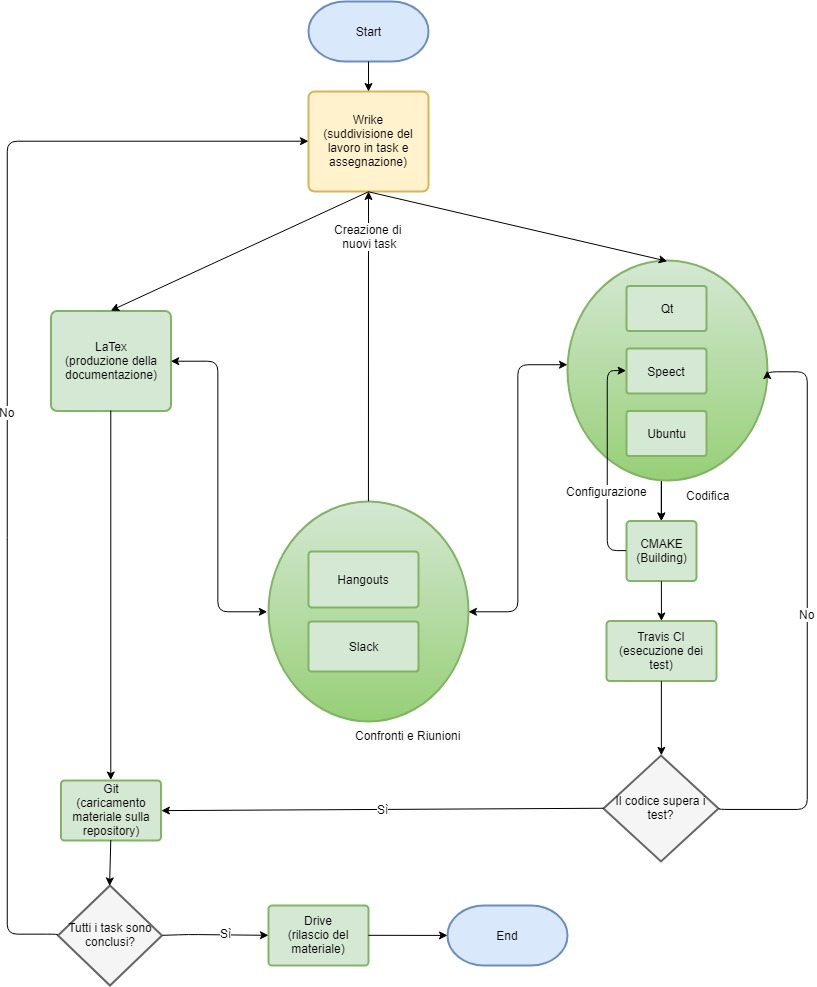
\includegraphics[scale=0.5]{tech-integration}
	\centering
	\caption{Schema riepilogativo dell'interazione delle tecnologie}
\end{figure}

\end{document}